 \section{Eksperimenti}

\subsection{Eksperimentalna postavka}

Svi eksperimenti sprovedeni su na javno dostupnom ViT-Base modelu sa veličinom 
peča 16 i ulaznom rezolucijom $224 \times 224$ piksela (\textit{ViT-Base/16-224}) 
\cite{dosovitskiy2021vit}, pretreniranom na skupu ImageNet-21k i fino podešenom 
na skupu ImageNet-1k. Model sadrži $L=12$ blokova enkodera, $h=12$ komponenata pažnje 
i prostornu dimenziju $D=768$, što ga čini standardnim referentnim modelom u 
literaturi za interpretabilnost Vision Transformer arhitektura.

Evaluacija je sprovedena na podskupu standardnog validacionog skupa ImageNet \cite{russakovsky2015imagenet}, koji ukupno sadrži $50000$ slika. Zbog ograničenja u pogledu vremena i računarskih resursa, evaluacija je izvršena na slučajno odabranom uzorku od $1000$ slika. Za potrebe procene lokalizacije korišćene su zvanične prostorne anotacije u obliku graničnih okvira (\textit{bounding boxes}), preuzete sa ImageNet platforme za anotaciju objekata. Na osnovu njih moguće je primeniti metrike lokalizacije opisane u nastavku.

Sve metode interpretabilnosti implementirane su u PyTorch okruženju i primenjene na identičnom skupu slika pod jednakim uslovima, čime se obezbeđuje fer poređenje. Svi proračuni i eksperimenti realizovani su uz korišćenje grafičkih procesora (\textit{GPU}) radi značajnog skraćenja vremena potrebnog za obradu podataka.

U pogledu prostorne rezolucije generisanih objašnjenja, u literaturi se metode poput \textit{Vanilla Gradient}, \textit{Gradient $\times$ Input} i \textit{LRP} često primenjuju direktno na ulazne piksele. Međutim, kako većina ostalih posmatranih metoda po svojoj prirodi radi u prostoru pečeva, u ovom radu su i metode zasnovane na gradijentima i propagaciji izračunate na nivou reprezentacije pečeva. Preciznije, propagacija signala značajnosti sprovedena je do \textit{patch embedding} \ref{sec:patch_emb} sloja, odnosno nad samim ulaznim tokenima enkodera. Ovim je postignuto da se mape za sve posmatrane metode dobijaju direktno u identičnoj prostornoj rezoluciji. Ovaj pristup ne samo da obezbeđuje potpunu metodološku doslednost pri proračunu metrika, već generiše i vizuelno jasnije mape značajnosti koje nisu opterećene visokofrekventnim šumom na nivou pojedinačnih piksela.

\subsection{Metrike evaluacije}

Evaluacija metoda interpretabilnosti predstavlja otvoren istraživački problem. 
Za razliku od standardnih zadataka mašinskog učenja gde postoji jasno definisana 
stvarna oznaka klase (\textit{ground-truth}), procena kvaliteta mapa značajnosti suočava se sa 
fundamentalnim izazovom — ne postoji jednoznačna definicija toga šta predstavlja 
ispravno objašnjenje. Dodatna poteškoća leži u tome što model i čovek 
mogu koristiti potpuno različite strategije za donošenje odluke o istoj slici, 
pa ljudska intuicija o važnim regionima ne mora nužno da odgovara onome što model 
zaista koristi tokom zaključivanja.

\subsubsection{MoRF i LeRF}

Metrike zasnovane na perturbaciji \cite{samek2017evaluating} pokušavaju da 
zaobiđu problem subjektivnosti uvođenjem automatizovane evaluacije koja ne 
zavisi od ljudske procene. Osnovna ideja je intuitivna: ako mapa značajnosti 
ispravno identifikuje ključne regione, uklanjanje tih regiona iz slike trebalo 
bi da dovede do bržeg pada tačnosti modela nego uklanjanje nasumičnih delova slike.

\textbf{MoRF} (\textit{Most Relevant First}) meri pad tačnosti modela kada 
se pečevi uklanjaju redom od najvažnijeg ka najmanje važnom prema mapi 
značajnosti. Formalno, neka je $\pi$ permutacija pečeva sortiranih prema 
opadajućoj vrednosti značajnosti, a $f_c(\mathbf{x}_{S_k})$ izlaz modela 
nakon što je uklonjeno prvih $k$ pečeva:

\begin{equation}
    \text{MoRF}(k) = f_c(\mathbf{x}_{S_k}), \quad 
    S_k = \{\pi(1), \ldots, \pi(k)\}
\end{equation}

Kvalitetnija metoda interpretabilnosti daje strmiji pad MoRF krive, što se 
kvantifikuje površinom ispod krive (\textit{Area Under Curve}, AUC) — 
niža vrednost AUC označava superiornije performanse metode.

\textbf{LeRF} (\textit{Least Relevant First}) predstavlja komplementarnu metriku 
koja uklanja pečeve redom od najmanje važnog ka najvažnijem. Kod ove metrike, 
viša vrednost AUC označava bolju metodu, jer pouzdana mapa značajnosti treba da sačuva 
tačnost modela što duže tokom uklanjanja irelevantnih regiona.

Obe metrike dele isto ograničenje — maskiranje i uklanjanje pečeva generiše 
slike koje odstupaju od trening distribucije modela (\textit{out-of-distribution}), 
što može nepredvidivo uticati na ponašanje mreže. Ovaj problem je delimično 
ublažen korišćenjem mehanizma maskiranja tokena opisanog u sekciji \ref{sec:masking}, 
koji ne modifikuje ulazne piksele već isključuje tokene direktno unutar mehanizma 
pažnje. Ipak, ovaj fenomen nije potpuno eliminisan jer model tokom treninga nije 
obučavan na slikama sa isključenim tokenima. 

U cilju smanjenja uticaja šuma koji 
nastaje usled ekstremne perturbacije ulaza, u ovom radu se pored standardne AUC metrike
analizira i delimični AUC ograničen na prvih $30\%$ uklonjenih pečeva, čime se 
evaluacija fokusira isključivo na najkritičnije regione slike.

Pored pojedinačnih AUC vrednosti, kao sintetička mera kvaliteta mape značajnosti 
koristi se i razlika LeRF $-$ MoRF. Intuicija je jednostavna: dobra metoda 
interpretabilnosti trebalo bi da generiše MoRF krivu koja strmije opada i LeRF 
krivu koja sporije opada u poređenju sa lošom metodom. Što je veća razlika između 
ove dve krive, to metoda preciznije razdvaja važne od nevažnih regiona. Ova 
kombinovana metrika omogućava direktno poređenje metoda jednim brojem, nezavisno 
od apsolutnih vrednosti tačnosti modela.

\subsubsection{Pointing Game}

Kako bi se evaluacija delimično uskladila sa ljudskom vizuelnom intuicijom o 
lokalizaciji objekata, primenjuje se \textit{Pointing Game} metrika 
\cite{zhang2018pointing}. Za svaku sliku identifikuje se koordinata sa 
maksimalnom vrednošću u mapi značajnosti i proverava se da li se ona nalazi 
unutar graničnog okvira (\textit{bounding box}) anotiranog objekta:

\begin{equation}
    \text{PG}(\mathbf{x}) = \mathbf{1}\left[ 
    \arg\max_{i,j} S(\mathbf{x})_{ij} \in \text{bbox}(\mathbf{x}) 
    \right]
\end{equation}

Ukupna tačnost lokalizacije na celom skupu dobija se usrednjavanjem pojedinačnih vrednosti:

\begin{equation}
    \text{Acc} = \frac{1}{|\mathcal{D}|} \sum_{\mathbf{x} \in \mathcal{D}} 
    \text{PG}(\mathbf{x})
\end{equation}

\textit{Pointing Game} je konceptualno jednostavna i lako interpretabilna metrika jer direktno meri sposobnost metode da lokalizuje objekat koji je čovek označio kao relevantan. 
Međutim, ona poseduje i određene nedostatke — izuzetno je osetljiva na mape značajnosti koje su 
ekstremno fokusirane na samo jedan piksel i ne uzima u obzir prostornu raspodelu 
važnosti van te tačke.

\subsubsection{Spirmanova korelacija}

Pored evaluacije apsolutnog kvaliteta svake pojedinačne metode, od ključnog je 
značaja ispitati i međusobnu sličnost mapa značajnosti dobijenih različitim metodama. 
Ukoliko dve metode daju visoko korelisane mape, to ukazuje na činjenicu da one 
detektuju slične aspekte ponašanja modela, bez obzira na njihove konceptualne razlike. 
Ova analiza je posebno relevantna za poređenje metoda zasnovanih na različitim teorijskim 
principima — visoka korelacija između metoda koje koriste potpuno različite izvore 
informacija sugeriše da one konvergiraju ka istom objašnjenju, dok niska korelacija 
otvara pitanje koja od njih vernije odražava stvarne procese unutar modela.

Sličnost mapa značajnosti kvantifikuje se preko Spirmanove korelacije ranga 
\cite{spearman1904}, koja je robusna na monotone transformacije vrednosti 
i ne zahteva pretpostavku o normalnosti raspodele:

\begin{equation}
    \rho = 1 - \frac{6 \sum_i d_i^2}{n(n^2-1)}
\end{equation}
gde $d_i$ predstavlja razliku rangova odgovarajućih elemenata (piksela ili pečeva) u dvema mapama značajnosti, 
dok je $n$ ukupan broj elemenata u mapi. Rezultati se prikazuju u formi matrice korelacije 
za sve parove metoda, usrednjene po celom evaluacionom skupu.

\subsubsection{Testovi specifični za Vision Transformer arhitekturu}

Pored standardnih metrika evaluacije, u ovom radu se predlažu dva dodatna 
testa motivisana specifičnostima same ViT arhitekture. Za razliku od prethodnih 
metrika koje mere apsolutni kvalitet mapa značajnosti, ovi testovi ispituju 
njihovu robusnost na perturbacije ulaza koje su usko povezane sa 
funkcionisanjem \textit{Transformer} modela.

\paragraph{Test globalnog mešanja pečeva.} Kao što je opisano u sekciji \ref{sec:posemb}, 
\textit{positional embeddings} se dodaju samo na početku mreže i 
predstavljaju jedini izvor prostorne informacije za model. Poznato je da 
ViT modeli mogu uspešno klasifikovati slike čak i kada su pečevi 
nasumično izmešani \cite{dosovitskiy2021vit}, što sugeriše da model 
donosi odluku primarno na osnovu semantičkog sadržaja samih pečeva, a ne njihovog prostornog 
rasporeda. Ovaj test ispituje u kojoj meri se taj fenomen odražava na mape značajnosti. 
U okviru testa, nasumično se permutuju svi pečevi ulazne slike, generiše se nova mapa 
značajnosti, a potom se meri njena Spirmanova korelacija sa originalnom mapom. 
Visoka korelacija ukazuje na to da metoda interpretabilnosti detektuje 
informacije koje nisu prostorno zavisne, što dodatno potvrđuje hipotezu da model 
donosi odluku na osnovu prisustva lokalnih karakteristika, a ne njihove globalne geometrije.

\paragraph{Test nasumičnog peča.} Mehanizam pažnje u ViT arhitekturi može posvetiti 
neproporcionalno veliku pažnju regionima koji odstupaju od trening distribucije 
jer ih model ne prepoznaje kao deo poznatog vizuelnog koncepta. Ovaj 
test ispituje navedenu hipotezu — na fiksnu poziciju unutar slike dodaje se peč sa 
slučajnim Gausovim šumom, koji je po definiciji van distribucije, 
nakon čega se meri Spirmanova korelacija mapa značajnosti pre i posle ove modifikacije. 
Niska korelacija ukazuje na to da metoda interpretabilnosti nije robusna na prisustvo 
šuma van distribucije, odnosno da se mapa značajnosti dramatično menja iako je sadržaj 
originalnih, relevantnih delova slike ostao netaknut. Posebno je interesantno ispitati 
razliku u robusnosti između metoda koje direktno propagiraju težine pažnje, poput 
metode \textit{Attention Rollout}, i onih koje ovaj signal ne posmatraju direktno, već se 
oslanjaju na analizu odnosa ulaza i izlaza.

\subsection{Rezultati}

\subsubsection{Vizuelno poređenje metoda}

Radi kvalitativne analize, mape značajnosti prikazane su za tri grupe 
primera koje pokrivaju različite scenarije od jednostavnih do složenih.

\paragraph{Jednostavni primeri.} Prva grupa (slika \ref{fig:good_examples}) 
obuhvata slike sa jasno istaknutim objektom — brod na otvorenom moru i krabu koja se ističe svojim karakterističnim kleštima. Na ovim primerima gotovo sve metode uspešno 
lokalizuju objekat od interesa, ali sa uočljivim razlikama u kvalitetu 
mapa. Attention Rollout pokazuje karakteristične artefakte rasute pažnje, 
dok gradijentne metode (Vanilla Gradient, Input $\times$ Gradient, GradCAM) 
prepoznaju objekat ali bez potpunog fokusiranja mape na njegovu celokupnu 
površinu. Kernel SHAP daje neujednačene mape sa sporadično istaknutim 
regionima. Transformer Attribution, RISE i GMAR pokazuju najkoherentnije 
rezultate sa mapama koje precizno pokrivaju objekat od interesa.

\begin{figure}[h]
    \centering
    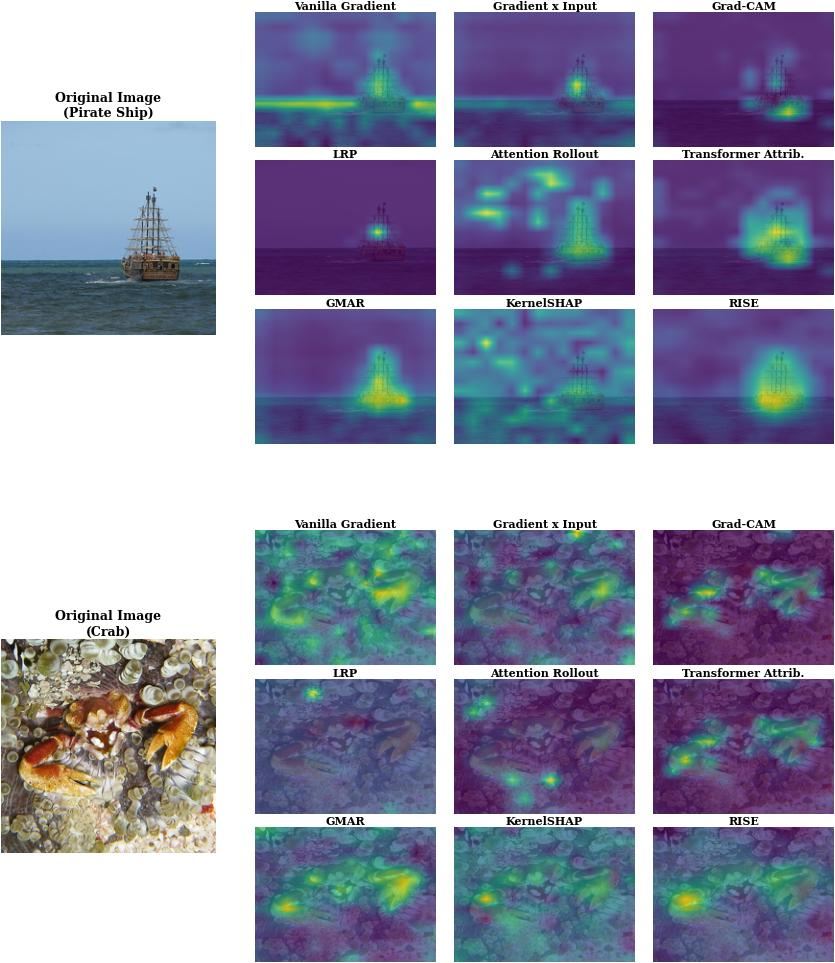
\includegraphics[width=0.75\textwidth]{figures/eval/good_examples2.jpg}
    \caption{Primeri sa jasno istaknutim objektom (brod na moru, kraba sa kleštima). Za svaku sliku prikazana je originalna slika (levo) 
    i mape značajnosti u formatu $3 \times 3$ (desno).}
    \label{fig:good_examples}
\end{figure}

\paragraph{Složeni primeri.} Druga grupa (slika \ref{fig:bad_examples}) 
obuhvata scenarije koji predstavljaju veći izazov za metode 
interpretabilnosti: mnoštvo instanci istog objekta (roj pčela), veliki 
objekat bez prepoznatljive teksture (monitor) i objekat koji se utapa 
u pozadinu (šipka za dizanje tegova). Kao što je i očekivano, rezultati 
su vidno lošiji u poređenju sa jednostavnim primerima, ali se između 
metoda uočavaju karakteristične razlike. RISE se posebno izdvaja kod 
monitora gde uspešno lokalizuje njegov nosač, dok Transformer 
Attribution daje najkoherentnije rezultate kod šipke koja se utapa u pozadinu.

\begin{figure}[H]
    \centering
    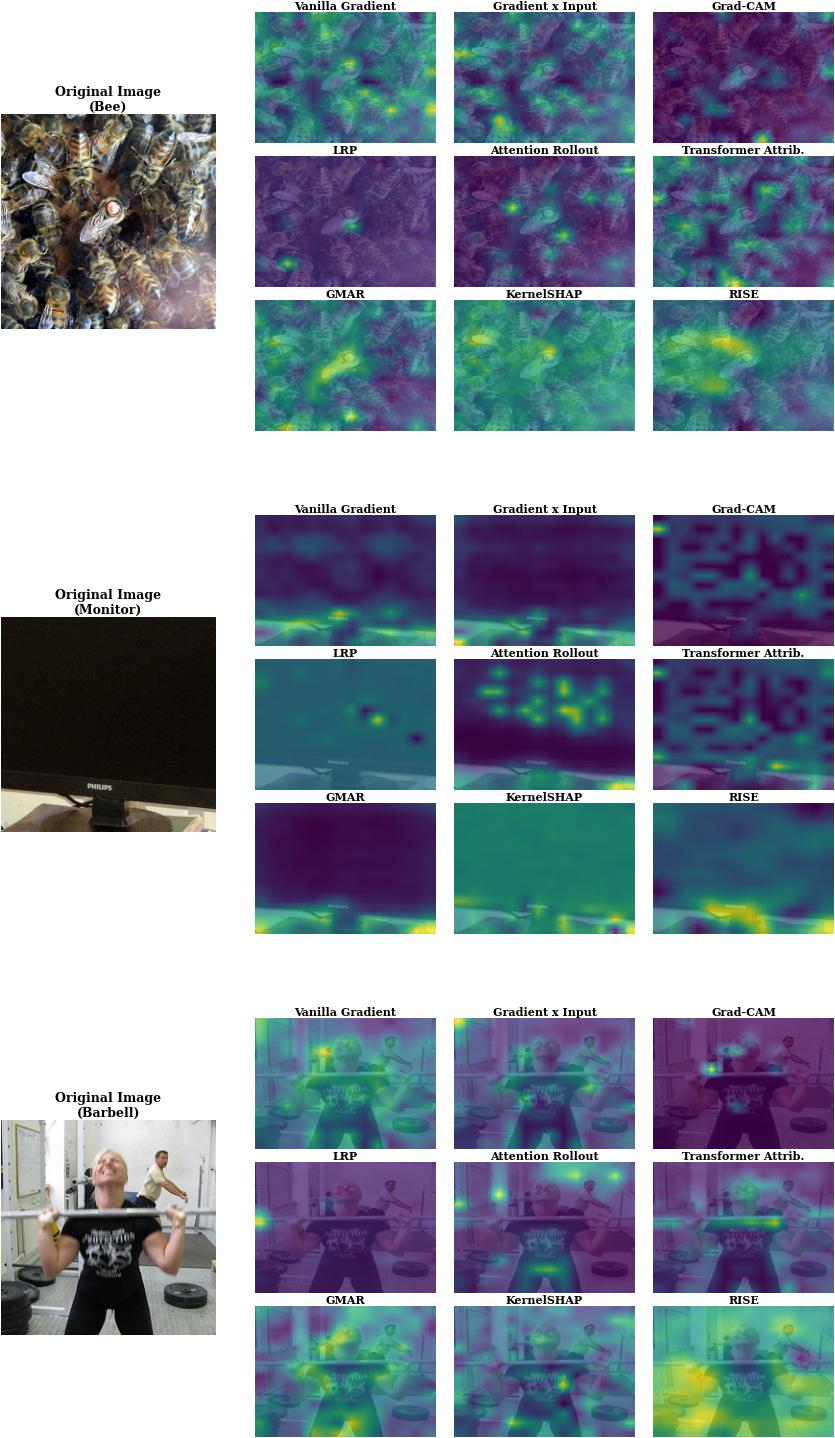
\includegraphics[width=0.75\textwidth]{figures/eval/bad_examples2.jpg}
    \caption{Složeni primeri: mnoštvo instanci objekta (roj pčela), 
    veliki objekat bez prepoznatljive teksture (monitor) i objekat koji 
    se utapa u pozadinu (šipka za dizanje tegova). Prikazane su originalna 
    slika (levo) i mape značajnosti u formatu $3 \times 3$ (desno).}
    \label{fig:bad_examples}
\end{figure}

\paragraph{Klasna diskriminativnost.} Treća grupa (slika \ref{fig:class_agnostic}) ispituje zavisnost mapa značajnosti od ciljne klase na dva primera: slici sa dva odvojena objekta (flandrijski govedar i haski) i sintetičkoj slici koja kombinuje telo zlatnog retrivera i glavu mačke. Klasno zavisne metode bi trebalo da fokusiraju pažnju na različite regione za različite ciljne klase. Rezultati pokazuju da Transformer Attribution, Kernel SHAP i RISE ispoljavaju jasnu klasnu diskriminativnost — mape značajnosti se vidno razlikuju u zavisnosti od klase. Ostale metode, uključujući i one zasnovane na gradijentima, u praksi ne ispoljavaju takvu doslednost.

\begin{figure}[H]
    \centering
    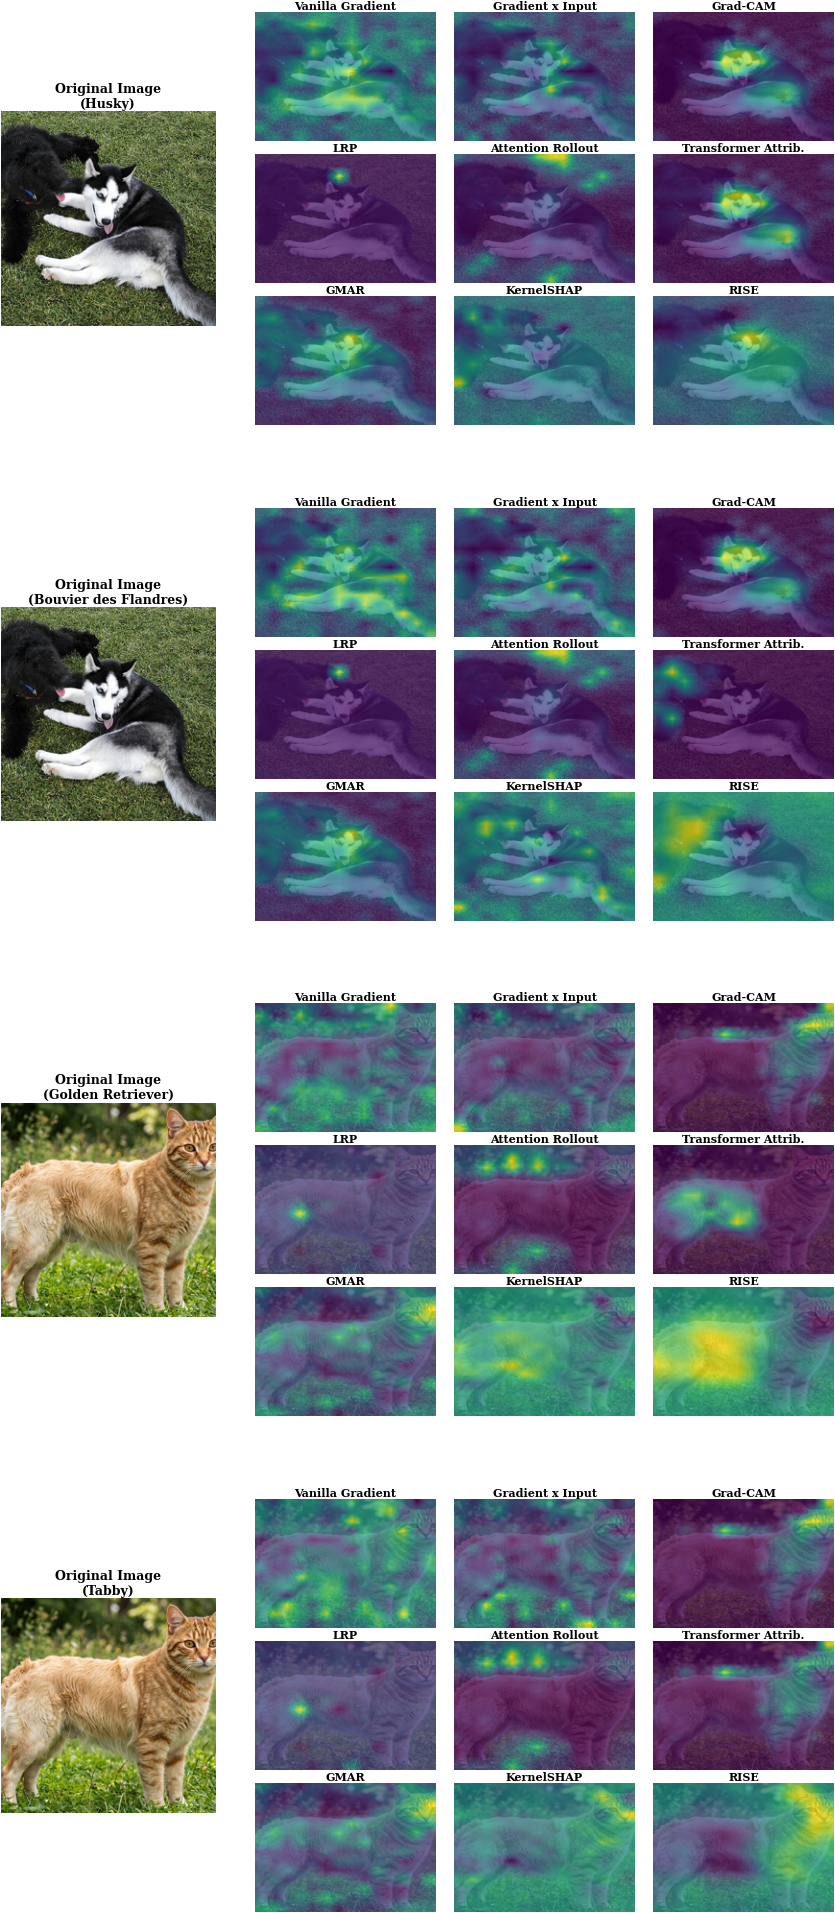
\includegraphics[width=0.48\textwidth]{figures/eval/class_agnostic2.png}
    \caption{Analiza klasne diskriminativnost: slika sa dve različite klase (flandrijski govedar i haski) i sintetička slika tela zlatnog retrivera sa glavom mačke. Mape su generisane za svaku klasu zasebno.}
    \label{fig:class_agnostic}
\end{figure}



\subsubsection{MoRF i LeRF}

\begin{table}[h]
\centering
\caption{MoRF i LeRF AUC vrednosti za sve metode. Niži MoRF AUC i 
viši LeRF AUC označavaju bolju lokalizaciju važnih regiona. 
AUC\textsubscript{30} označava vrednost računatu na prvih 30\% 
uklonjenih pečeva.}
\label{tab:morf_lerf}
\begin{tabular}{llcccc}
\hline
\textbf{Grupa} & \textbf{Metoda} & \textbf{MoRF} & \textbf{MoRF\textsubscript{30}} & \textbf{LeRF} & \textbf{LeRF\textsubscript{30}} \\
\hline
\multirow{3}{*}{Gradijentne}
    & Vanilla Gradient        & $0.518$ & $0.712$ & $0.594$ & $0.732$ \\
    & Input $\times$ Gradient & $0.515$ & $0.714$ & $0.591$ & $0.731$ \\
    & GradCAM                 & $0.456$ & $0.620$ & $0.615$ & $0.739$ \\
\hline
    & LRP                     & $0.537$ & $0.710$ & $0.600$ & $0.730$ \\
\hline
\multirow{3}{*}{Mehanizam pažnje}
    & Attention Rollout       & $0.515$ & $0.701$ & $0.555$ & $0.730$ \\
    & Transformer Attribution & $0.326$ & $0.574$ & $0.660$ & $0.742$ \\
    & GMAR                    & $0.418$ & $0.655$ & $0.628$ & $0.736$ \\
\hline
\multirow{2}{*}{Ulaz/izlaz}
    & Kernel SHAP             & $0.494$ & $0.657$ & $0.616$ & $0.758$ \\
    & \textbf{RISE}           & $\mathbf{0.198}$ & $\mathbf{0.437}$ & $\mathbf{0.846}$ & $\mathbf{0.824}$ \\
\hline
\end{tabular}
\end{table}

\begin{table}[h]
\centering
\caption{Razlika LeRF $-$ MoRF AUC. Veća vrednost ukazuje na bolju 
sposobnost razlikovanja važnih od nevažnih regiona.}
\label{tab:lerf_morf}
\begin{tabular}{llcc}
\hline
\textbf{Grupa} & \textbf{Metoda} & \textbf{LeRF $-$ MoRF} & \textbf{LeRF\textsubscript{30} $-$ MoRF\textsubscript{30}} \\
\hline
\multirow{3}{*}{Gradijentne}
    & Vanilla Gradient        & $0.076$ & $0.020$ \\
    & Input $\times$ Gradient & $0.076$ & $0.017$ \\
    & GradCAM                 & $0.159$ & $0.119$ \\
\hline
    & LRP                     & $0.063$ & $0.020$ \\
\hline
\multirow{3}{*}{Mehanizam pažnje}
    & Attention Rollout       & $0.040$ & $0.029$ \\
    & Transformer Attribution & $0.334$ & $0.168$ \\
    & GMAR                    & $0.210$ & $0.081$ \\
\hline
\multirow{2}{*}{Ulaz/izlaz}
    & Kernel SHAP             & $0.122$ & $0.101$ \\
    & \textbf{RISE}           & $\mathbf{0.648}$ & $\mathbf{0.387}$ \\
\hline
\end{tabular}
\end{table}

\begin{figure}[h]
    \centering
    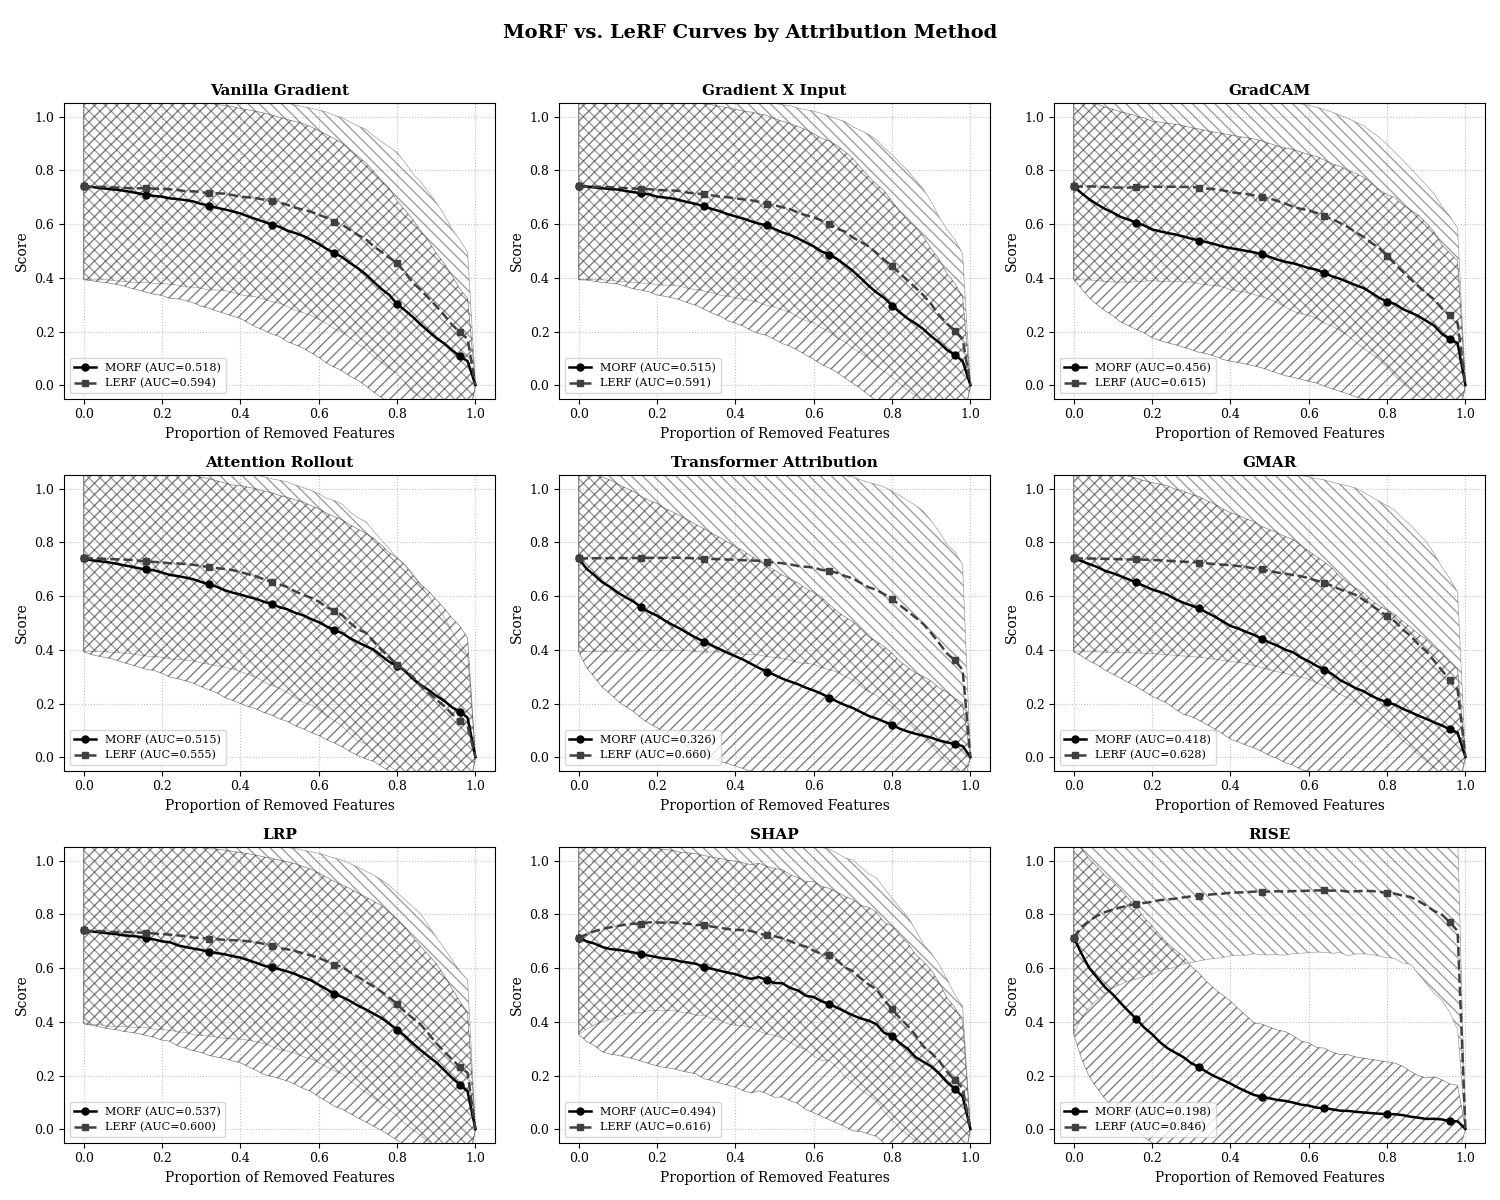
\includegraphics[width=0.9\textwidth]{figures/eval/morf_lerf_bw.png}
    \caption{MoRF i LeRF krive za sve evaluirane metode. Na svakom 
    grafikonu prikazana je zavisnost tačnosti modela od udela uklonjenih 
    pečeva, sa standardnom devijacijom. Strmiji pad MoRF krive i sporiji 
    pad LeRF krive označavaju bolju metodu.}
    \label{fig:morf_lerf_curves}
\end{figure}

Kvantitativni rezultati (Tabela \ref{tab:lerf_morf}) potvrđuju superiornost RISE metode, koja postiže ubedljivo najveću razliku LeRF $-$ MoRF ($0.648$), pokazujući izuzetnu preciznost u razdvajanju relevantnih od irelevantnih regiona. Među ostalim metodama ističe se Transformer Attribution (razlika $0.334$), dok sirove mape pažnje (Attention Rollout) beleže najlošiji rezultat od svih metoda ($0.040$).

Gradijentne metode i LRP pokazuju malu razliku između MoRF i LeRF vrednosti, što ukazuje na njihovu slabu sposobnost rangiranja važnosti pečeva. Uprkos generisanju vizuelno razmazanih mapa, Kernel SHAP ostvaruje zadovoljavajući kvantitativni rezultat ($0.122$), čime se potvrđuje da vizuelni kvalitet mapa nije nužno u korelaciji sa tačnošću lokalizacije.


\subsubsection{Pointing Game}

\begin{table}[H]
\centering
\caption{Preciznost lokalizacije prema metrici \textit{Pointing Game} 
na 1000 slika validacionog skupa.}
\label{tab:pointing_game}
\begin{tabular}{llc}
\hline
\textbf{Grupa} & \textbf{Metoda} & \textbf{Preciznost (\%)} \\
\hline
\multirow{3}{*}{Gradijentne}
    & Vanilla Gradient        & $66.0$ \\
    & Input $\times$ Gradient & $62.8$ \\
    & GradCAM                 & $70.2$ \\
\hline
    & LRP                     & $62.2$ \\
\hline
\multirow{3}{*}{Mehanizam pažnje}
    & Attention Rollout       & $42.9$ \\
    & Transformer Attribution & $84.4$ \\
    & GMAR                    & $76.8$ \\
\hline
\multirow{2}{*}{Ulaz/izlaz}
    & Kernel SHAP (8k maski)  & $62.6$ \\
    & RISE (6k maski)         & $\mathbf{85.7}$ \\
\hline
\end{tabular}
\end{table}

Rezultati \textit{Pointing Game} metrike pokazuju da RISE postiže najbolju preciznost lokalizacije ($85.7\%$), a blisko ga prati Transformer Attribution ($84.4\%$). Na drugom kraju spektra, Attention Rollout beleži najlošiji rezultat ($42.9\%$), što ukazuje na to da sirovi težinski koeficijenti pažnje nisu pouzdani indikatori lokalizacije.

Gradijentne metode i LRP ostvaruju umerene rezultate u opsegu $62.2\%$--$70.2\%$.
Kernel SHAP postiže svega $62.6\%$, što potvrdjuje da formalne aksiomatske garancije ne garantuju dobru prostornu lokalizaciju kada se analiza vrši na nivou grubih pečeva.

\subsubsection{Spirmanova korelacija između metoda}

\begin{figure}[h]
    \centering
    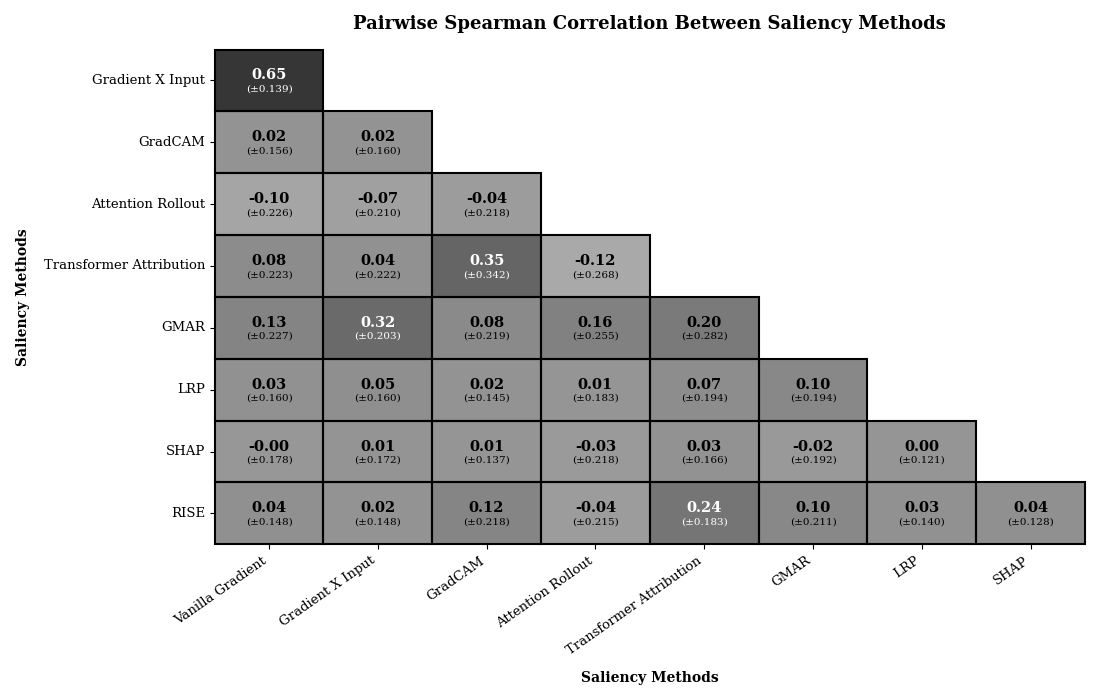
\includegraphics[width=0.8\textwidth]{figures/eval/spearman_correlation_bw.png}
    \caption{Matrica Spirmanove korelacije između mapa značajnosti 
    svih parova metoda, usrednjena po validacionom skupu.}
    \label{fig:spearman_matrix}
\end{figure}

Analiza Spirmanove korelacije otkriva da su mape značajnosti različitih metoda u velikoj meri međusobno nezavisne. Jedina značajna korelacija uočava se između Vanilla Gradient i Input $\times$ Gradient ($\rho = 0.65$), 
što je očekivano s obzirom da druga metoda predstavlja direktnu nadogradnju prve. Umerena korelacija postoji i između GradCAM i Transformer Attribution 
($\rho = 0.35$) kao i između Input $\times$ Gradient i GMAR ($\rho = 0.32$).

Primećuje se da Kernel SHAP praktično nije u korelaciji ni sa jednom metodom ($|\rho| < 0.05$ za sve parove), što u kombinaciji sa lošim rezultatima na ostalim metrikama sugeriše da ova metoda ne konvergira ka smislenim mapama značajnosti. Attention Rollout 
jedini pokazuje negativnu korelaciju sa gradijentnim metodama i Transformer Attribution, što je u skladu sa njegovim lošim kvantitativnim rezultatima.

\subsubsection{Testovi specifični za Vision Transformer arhitekturu}

\begin{table}[h]
\centering
\caption{Spirmanova korelacija mapa značajnosti pre i posle perturbacije ulaza ($\rho \pm \sigma$). Viši $\rho$ označava veću robustnost metode.}
\label{tab:robustness}
\resizebox{\textwidth}{!}{%
\begin{tabular}{llcccc}
\hline
\textbf{Grupa} & \textbf{Metoda} & \textbf{Shuffle} & 
\makecell{\textbf{Perturb} \\ \textbf{(najvažniji)}} & 
\makecell{\textbf{Perturb} \\ \textbf{(najmanje važan)}} & 
\makecell{\textbf{Perturb} \\ \textbf{(nasumični)}} \\
\hline
\multirow{3}{*}{Gradijentne}
    & Vanilla Gradient        & $0.227$ & $0.876$ & $0.901$ & $0.898$ \\
    & Input $\times$ Gradient & $0.412$ & $0.909$ & $0.940$ & $0.935$ \\
    & GradCAM                 & $0.047$ & $0.871$ & $0.930$ & $0.946$ \\
\hline
    & LRP                     & $0.025$ & $0.031$ & $0.045$ & $0.034$ \\
\hline
\multirow{3}{*}{Mehanizam pažnje}
    & Attention Rollout       & $0.367$ & $0.982$ & $0.988$ & $0.988$ \\
    & Transformer Attribution & $0.298$ & $0.908$ & $0.909$ & $0.911$ \\
    & GMAR                    & $\mathbf{0.727}$ & $\mathbf{0.987}$ & $\mathbf{0.996}$ & $\mathbf{0.995}$ \\
\hline
\multirow{2}{*}{Ulaz/izlaz}
    & Kernel SHAP             & $0.565$ & $0.893$ & $0.896$ & $0.900$ \\
    & RISE                    & $0.037$ & $0.845$ & $0.849$ & $0.858$ \\
\hline
\end{tabular}%
}
\end{table}

\paragraph{Test globalnog mešanja pečeva.} GMAR pokazuje izuzetno visoku 
robustnost na globalni raspored pečeva ($\rho = 0.727$), što sugeriše 
da ova metoda generiše mape koje su u velikoj meri nezavisne od prostornog 
rasporeda — isti pečevi se ističu bez obzira na njihovu poziciju u slici. 
Kernel SHAP pokazuje umerenu robustnost ($\rho = 0.565$), dok GradCAM, 
LRP i RISE pokazuju minimalnu korelaciju nakon mešanja ($\rho < 0.05$), 
što znači da su njihove mape izrazito prostorno zavisne.

\paragraph{Test nasumičnog peča.} LRP se izdvaja kao izrazito osetljiva 
metoda — korelacija praktično pada na nulu ($\rho \approx 0.03$) za sve 
tri varijante perturbacije, što znači da dodavanje jednog nasumičnog peča 
potpuno menja mapu značajnosti. Ovo sugeriše da LRP propagacija relevantnosti 
kroz sve slojeve mreže čini metodu izrazito osetljivom na lokalne promene 
ulaza. Nasuprot tome, Attention Rollout i GMAR pokazuju izuzetnu robustnost 
($\rho > 0.98$), što potvrđuje da mape zasnovane na mehanizmu pažnje nisu osetljive na prisustvo pojedinačnih pečeva van očekivane distribucije.

\subsubsection{Vremena izvršavanja}

Tabela \ref{tab:timing} prikazuje prosečno vreme izvršavanja po slici 
za sve evaluirane metode, mereno na GPU akceleratoru.

\begin{table}[h]
\centering
\caption{Prosečno vreme izvršavanja po slici.}
\label{tab:timing}
\begin{tabular}{llccc}
\hline
\textbf{Grupa} & \textbf{Metoda} & \textbf{$\mu$} & \textbf{$\sigma$} & \textbf{Jedinica} \\
\hline
\multirow{3}{*}{Gradijentne} 
    & Vanilla Gradient        & $44.69$ & $5.03$  & ms \\
    & Input $\times$ Gradient & $45.81$ & $6.82$  & ms \\
    & GradCAM                 & $30.18$ & $4.69$  & ms \\
\hline
    & LRP                     & $180.57$ & $14.51$ & ms \\
\hline
\multirow{3}{*}{Mehanizam pažnje}
    & Attention Rollout       & $18.36$  & $2.62$  & ms \\
    & Transformer Attribution & $212.27$ & $16.35$ & ms \\
    & GMAR                    & $48.62$  & $4.31$  & ms \\
\hline
\multirow{2}{*}{Ulaz/izlaz}
    & Kernel SHAP (8k maski)  & $52.58$ & $1.22$ & s \\
    & RISE (6k maski)         & $38.62$ & $0.52$ & s \\
\hline
\end{tabular}
\end{table}

Attention Rollout je ubedljivo najbrža metoda ($18.36$ ms) jer ne zahteva  prolaz unazad kroz mrežu. Transformer Attribution je najsporija  metoda koja poznaje strukturu modela ($212.27$ ms) zbog računanja gradijenata i relevantnosti po matricama pažnje za 
svaki sloj. Metode zasnovane na analizi ulaza i izlaza su za dva do tri reda veličine sporije od ostalih — Kernel SHAP zahteva $52.58$ s a RISE $38.62$ s po slici, što ih čini nepraktičnim za primenu u realnom vremenu uprkos konkurentnim kvantitativnim rezultatima.
\newpage
\subsection{Diskusija}

Rezultati eksperimentalne evaluacije omogućavaju sistematično poređenje 
metoda interpretabilnosti kroz nekoliko dimenzija: kvalitet lokalizacije, 
računarska efikasnost, robustnost i klasna diskriminativnost.

\paragraph{Metode zasnovane na mehanizmu pažnje.}
Attention Rollout, iako ubedljivo najbrža metoda ($18.36$ ms), pokazuje 
konzistentno loše rezultate na svim kvantitativnim metrikama — najniži 
\textit{Pointing Game} ($42.9\%$), minimalna razlika LeRF $-$ MoRF 
($0.040$) i negativna korelacija sa većinom ostalih metoda. Ovo potvrđuje 
teorijska ograničenja diskutovana u poglavlju o metodama — sirove mape 
pažnje nisu pouzdan signal važnosti regiona, a jednostavno množenje 
matrica kroz slojeve pojačava artefakte umesto da ih eliminiše. Brzina 
metode ne kompenzuje njen loš kvalitet.

GMAR se, nasuprot tome, pokazuje kao najbolji kompromis između kvaliteta 
i efikasnosti među metodama sa pristupom modelu. Uz vreme izvršavanja od 
$48.62$ ms, postiže solidne rezultate na svim metrikama i posebno se 
izdvaja u testovima robustnosti — sa $\rho = 0.727$ na testu mešanja 
pečeva i $\rho > 0.98$ na testu nasumičnog peča, GMAR je ubedljivo 
najrobusnija metoda. Ovo sugeriše da ponderisanje komponenti pažnje gradijentnim signalom ne samo da poboljšava kvalitet mapa već i stabilizuje njihov odgovor na perturbacije ulaza.

Transformer Attribution postiže odlične ukupne rezultate — drugi najbolji 
\textit{Pointing Game} ($84.4\%$) i drugu najveću razliku LeRF $-$ MoRF 
($0.334$) — ali po cenu skoro četiri puta dužeg vremena izvršavanja u 
odnosu na GMAR ($212.27$ ms). Mape koje ova metoda generiše su vizuelno 
najčistije i semantički najkoherentnije. Stoga, ukoliko je vreme izvršavanja 
kritičan faktor, GMAR predstavlja prirodan izbor, dok Transformer 
Attribution dolazi do izražaja kada je kvalitet mapa primarni cilj.

\paragraph{Gradijentne metode.}
Vanilla Gradient i Input $\times$ Gradient pokazuju ujednačene i umerene 
rezultate na svim metrikama, bez jasne prednosti jedne nad drugom uprkos 
teorijskoj motivaciji za uvođenje ulaza kao korekcije. Obe metode tehnički 
mogu operisati na nivou piksela, ali na slikama ovo nije prednost — 
prostorna korelacija susednih piksela uzrokuje šumovite i teško 
interpretabilne mape. GradCAM se pokazuje nešto boljim izborom u odnosu na Vanilla Gradient 
i Input $\times$ Gradient. Za razliku od ovih metoda koje propagiraju 
gradijent sve do ulaznog sloja kroz sve nelinearnosti mreže, GradCAM 
koristi gradijente po aktivacijama dubokih slojeva koji su semantički 
bogatiji i manje izloženi kumulativnom efektu višestrukih nelinearnih 
transformacija. Ipak, ni ova metoda ne dostiže kvalitet metoda zasnovanih na mehanizmu pažnje.

\paragraph{LRP.}
LRP se pokazuje kao najproblematičnija metoda u ovoj eksperimentalnoj postavci. 
Pored lošijih rezultata na standardnim metrikama, ova metoda pokazuje 
neočekivano ponašanje u testovima robustnosti — korelacija sa originalnom 
mapom pada praktično na nulu ($\rho \approx 0.03$) pri dodavanju jednog 
nasumičnog peča, što je drastično lošije od svih ostalih metoda. Ovo 
sugeriše da propagacija relevantnosti kroz sve slojeve mreže čini metodu 
izrazito osetljivom na lokalne promene ulaza — jedna perturbacija menja 
tok relevantnosti kroz celu mrežu, što rezultuje potpuno drugačijim mapama. 
Iz tog razloga LRP bi trebalo koristiti sa oprezom u praktičnim primenama.

\paragraph{Metode crne kutije.}
RISE se pokazuje kao ubedljivo najbolja metoda na MoRF/LeRF metrikama (MoRF AUC $0.198$, LeRF $-$ MoRF $0.648$) i postiže najbolji \textit{Pointing Game} rezultat ($85.7\%$) od svih evaluiranih metoda. Međutim, cena ovog kvaliteta je 
vreme izvršavanja od $38.62$ sekundi po slici — za dva do tri reda 
veličine sporije od prethodno pomenutih metoda. U scenarijima gde nema pristupa modelu, RISE predstavlja pouzdan izbor, ali je nepraktičan za primene koje zahtevaju brzu obradu.

Kernel SHAP, uprkos formalnoj aksiomatskoj osnovi Shapley vrednosti, 
pokazuje loše rezultate na gotovo svim metrikama i praktično nultu 
korelaciju sa svim ostalim metodama. Ovo ukazuje da matematički 
formalizam sam po sebi nije dovoljan garant kvaliteta — ograničena 
rezolucija peč reprezentacije i sporija konvergencija Shapley aproksimacije čine ovu metodu nepogodnom za interpretabilnost slika u poređenju sa metodom RISE.

\paragraph{Vizuelne karakteristike mapa.}
Jasna razlika između metoda sa i bez pristupa modelu ogleda se u samoj prirodi mapa značajnosti. Metode sa pristupom modelu, a naročito one zasnovane na mehanizmu pažnje, imaju tendenciju ka binarnijem prikazu — region od interesa je oštro istaknut, dok se pozadina tretira kao potpuno irelevantna. Ovakvo ponašanje je direktna posledica uzimanja u obzir isključivo pozitivnih doprinosa ($z^+$  pravilo i pozitivni gradijenti) što polarizuje mape i vodi ka ekstremnim vrednostima. S druge strane, metode bez pristupa modelu generišu mape sa glađim prelazima, gde je region od interesa naglašen, ali pozadina nije u potpunosti zanemarena. To može predstavljati značajnu prednost u situacijama u kojima širi kontekst scene utiče na konačnu odluku modela.

\paragraph{Klasna diskriminativnost.} 
Analiza ponašanja metoda na slikama sa prisustvom objekata iz dve različite klase ukazala je na interesantan fenomen. Sa teorijskog stanovišta, svaka metoda oslonjena na gradijentni signal ciljne klase trebalo bi da reprodukuje različite mape za različite klase, usled eksplicitnog izračunavanja gradijenta u odnosu na zadatu klasu. Ipak, usled propagacije unazad kroz duboku arhitekturu mreže, gradijentni signal postepeno gubi svoju klasnu specifičnost. Posmatrajući metode sa pristupom modelu, isključivo Transformer Attribution zadržava visoku klasnu osetljivost. To se postiže eksplicitnim ponderisanjem relevantnosti gradijentom ciljne klase direktno na matricama pažnje, zaobilazeći na taj način slabljenje signala kroz slojeve. Nasuprot tome, pristupi zasnovani na crnoj kutiji (Kernel SHAP, RISE) postižu klasnu diskriminativnost alternativnim putem — usmeravanjem procene važnosti ka relevantnim regionima kroz direktnu evaluaciju modela za željenu klasu u svakom iterativnom prolasku unapred.

\paragraph{Međusobna sličnost metoda.} 
Uočene niske vrednosti Spirmanove korelacije sugerišu da različite metode kvantifikuju suštinski različite aspekte ponašanja modela. Iako navedeno odstupanje nije neočekivano usled konceptualnih razlika između analiziranih pristupa, ono ukazuje na ozbiljno praktično ograničenje. Konkretno, nedostatak opšteg slaganja metoda pri detekciji relevantnih regiona otežava formulisanje pouzdanih zaključaka ukoliko se koristi isključivo jedna metoda.